\title{ {\bf Elliptic Curve Cryptosystems}}
\author{
          \text{S}\text{an}\text{ti}\text{ag}o \text{P}\text{ai}\text{va}\\
	  \small{{\tt \text{s}\text{an}\text{t}\text{ia}\text{go.p}\text{a}\text{iv}\text{a@m}\text{ai}\text{l.m}\text{cgi}ll\text{.}ca}}\\ \\
               \text{Mc}\text{Gill} \text{Uni}\text{ver}\text{sity}
          }
\date{April 25th, 2013}

\documentclass[12pt]{article}

\usepackage{amsmath}
\usepackage{amssymb}
\usepackage{amsthm}
\usepackage{color}
\usepackage{graphicx}
\usepackage{mnsymbol}
\usepackage{enumerate}
\setlength{\textwidth}{5.5in}
\setlength{\textheight}{8in}
\newcommand{\h}[1]{\colorbox{yellow}{#1}}
\newcommand{\problem}{\subsection*}
\newcommand{\R}{\mathbb{R}}
\newcommand{\F}{\mathbb{F}}
\newcommand{\Z}{\mathbb{Z}}
\newcommand{\Q}{\mathbb{Q}}
\newcommand{\C}{\mathbb{C}}
\newcommand{\Oo}{\mathcal{O}}

\begin{document}
\maketitle

%----------------------------------------------------------------------------------------
%	ABSTRACT
%----------------------------------------------------------------------------------------

\begin{abstract}

\noindent The application of elliptic curves in the field of cryptography has significantly improved the possibilities of security, encryption, and real-world applications. In this paper, we want to give a short introduction to Elliptic Curve Cryptosystems (ECC). The paper will start with some motivation behind the study of elliptic curves, followed by some essential concepts and background material. We will then discuss the discrete logarithm problem using elliptic curves, followed by a brief description of different cryptosystems, and we will finally conclude with a basic application of elliptic curves using PARI. 

\end{abstract}

%----------------------------------------------------------------------------------------
%	ARTICLE CONTENTS
%----------------------------------------------------------------------------------------


\section{Motivation behind elliptic curves}

We begin this section by describing the motivation behind the study of elliptic curves. Elliptic curves have been studied for quite a long time in Number Theory, but the application of elliptic curves to the field of cryptography is a recent phenomenon. \\

The reason elliptic curves are interesting mathematical objects is because the solutions form an Abelian group.  This means that we can ``add" two points on the curve and get another point on the curve.  This addition is associative, commutative, and has an identity and inverses. \\

Elliptic curves sometimes arise in the study of Diophantine Equations, which means that given an equation, we want to find all integer, or all rational, solutions.  There are methods for solving this kind of problem on elliptic curves, but no algorithm is known that will demostrably solve all these equations.\\

There are related algorithms for testing and verifying that a large number is prime using elliptic curves. What is special about elliptic curves is that there are cryptographic schemes that work on elliptic curves that are more secure and more efficient than similar codes that only use regular modular arithmetic.  \\

Faced with an infinite variety of elliptic curves to choose from, extensive research has been placed on how different cryptosystems using different elliptic curves perform. In this paper, we turn our attention to a major computationally hard problem in Number Theory: the so-called Discrete Logarithm Problem. Basically, we want to understand how can we efficiently compute $\log_gb$? No efficient classical algorithm for computing the general discrete logarithm is known. 

\section{Introduction and Background Material}

\subsection{Basics of Elliptic Curves}

We now introduce the notion of elliptic curves. Let $K$ be a field. In this paper, $K$ will be either the field $\R$ of real numbers, the field $\Q$ of rational numbers, the field $\C$ of complex numbers, or the finite field $\F_q$ of $q=p^r$ elements. The following definition is taken from [Ko].\\

{\bf Definition.} Let $K$ be a field of characteristic  $\neq 2,3$ and let $x^3 + ax + b$, where $a,b \in K$, be a cubic polynomial with no multiple roots. Then, an \emph{Elliptic Curve over K}, noted as $E(K)$, is defined to be the set of points $(x,y)$ with $x,y \in K$, satisfying the equation\footnote[1]{This type of equation is called a ``Weierstrass equation".}: 

\begin{equation}
y^2 = x^3 + ax + b\;
\end{equation}

together with a single element denoted $\mathcal{O}$ called the ``point at infinity". \\

\begin{itemize}
\item If $K$ is a field of characteristic 2, then an elliptic curve over $K$ is the set of points satisfying an equation of the following type:

\begin{equation}
y^2 + cy = x^3+ax+b \;\;\;\;\;\;\;\;\;\;\; y^2+xy = x^3 + ax^2 +b
\end{equation}

(where the cubic on the right has no multiple roots) together with $\mathcal{O}$ \\

\item If $K$ is a field of characteristic 3, then an elliptic curve over $K$ is the set of points satisfying the equation 
\end{itemize}

\begin{equation}
y^2 = x^3 + ax^2 +bx + c
\end{equation}

\noindent We now procede to discuss examples of elliptic curves over various fields: \\

\noindent {\bf Elliptic curves over $\R$.}\\

We introduce a centrally important fact about the set of points on an elliptic curve: they form an Abelian group! \\

The following definition comes from [Si].\\

\noindent {\bf Definition.} Let $E$ be an elliptic curve over the real numbers, and let $P$ and $Q$ be two points on $E$. We define the negative of $P$ and the sum $P+Q$ according to the following rules: 

\begin{enumerate}
\item If $P$ is the point at $\Oo$, then we define $-P$ to be $\Oo$ and $P+Q$ to be $Q$; i.e., $\Oo$ serves as the additive indentity, or zero element, of the group of points. 
\item The negative $-P$ is the point with the same $x$-coordinate but negative $y$-coordinate of $P$. That is, $-(x,y) = (x,-y)$. It follows from (1) that $(x,-y)$ is on the curve whenever $(x,y)$ is also on the curve. 
\item If $P$ and $Q$ have different $x$-coordinates, then it is not hard to see that the line $l = \overline{PQ}$ intersects the curve in exactly one more point $R$ (unless that line is tangent to the curve at $P$, in which case we take $R=P$, or at $Q$, in which case we take $R=Q$). Then, define $P+Q$ to be $-R$, the mirror image (with respect to the $x$-axis) of the third point of intersection.
\item If $Q = -P$, then we define $P+Q = \Oo$
\item If $P = Q$, then let $l$ be the tangent line to the curve at $P$, let $R$ be the only other point of intersection of $l$ with the curve, and define $P+Q = -R$. ($R$ is taken to be $P$ if the tanget line has a ``double tangency" at $P$, i.e., if $P$ is a point of inflection.)
\end{enumerate}
 
\begin{figure}
\caption{A graphic representation of an elliptic curve addition over $\R$.}
  \centering
  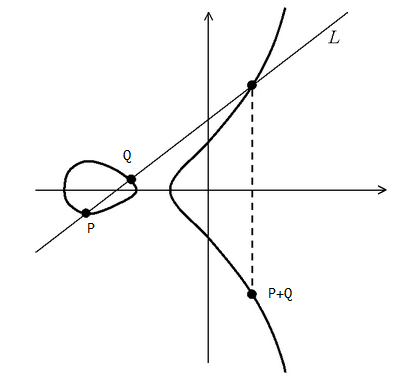
\includegraphics[width=0.5\textwidth]{ellipticcurve.png}
\end{figure}

\noindent {\bf Elliptic curves over $\C$.}\\

The algebraic formulas (4) and (5) for adding points on an elliptic curve over the reals actually make sense over any field. It can be shown that these formulas give an abelian group law on an elliptic curve over any field\footnote[2]{Not shown in this paper. The only hard part is to show associativity}.  \\

Let $E$ be an elliptic curve defined over $\C$. We have that $E$ is the set of pairs $(x,y)$ of complex numbers satisfying: $y^2 = x^3 + ax + b$, together with the point at infinity $\Oo$. Although $E$ is a ``curve", it is two-dimensional, i.e., it is a surface in the 4-real-dimensional space whose coordinates are the real and imaginary part of $x$ and $y$. [Ko] \\

We now describe how $E$ can be visualized as a surface: \\

The following definition is taken from [Si].\\

\noindent {\bf Definition.} Let $L$ be a \emph{lattice} in the complex plane. This means that $L$ is the abelian group of all integer combinations of two complex numbers $\omega_1$ and $\omega_2$, where $\omega_1$ and $\omega_2$ span the plane. Then, 

\begin{displaymath}
L = \Z\omega_1 + \Z\omega_2
\end{displaymath}

For example, if $\omega_1 = 1$ and $\omega_2 = \imath$, then $L$ is the Gaussian integers, the square grid of all complex numbers with integer real and imaginary parts. \\

To vizualize this, folding over one side of the parallelogram to meet the opposite side and then folding over again and gluing the opposite circles, we see that we obtaine a donut-like shape we call a ``torus."\\


\noindent {\bf Elliptic curves over $\F_q$.} \\

Let $K$ be the finite field $\F_q$ of $q = p^r$ elements. Let $E$ be an elliptic curve defined over $\F_q$. If $p=2,3$, then $E$ is given by an equation of the form (2) or (3). \\

It is easy to see that an elliptic curve can have at most $2q+1\;\F_q$ points, i.e., the point at infinity along with $2q$ pairs $(x,y)$ with $x,y \in \F_q$ which satisfy (1), or (2) if $p=2$ or (3) if $p=3$. Namely, for each of the $q$ possible $x$'s there are at most 2 $y$'s which satisfy (1). \\

But since only half of the elements of $\F_q^{\times}$ have square roots, one would expect (if $x^3 + ax + b$ were random elements of the field) that there would be only about half of that number of $\F_q$ points.  More precisely, let $\chi$ be the quadratic character of $\F_q$.  This is a map which takes $x \in F_{q}^{\times}$ to $\pm 1$ depending on whether or not $x$ has a square root in $\F_q$ (and we take $\chi(0) = 0$) [Si]. \\

For example, if $q = p$ is a prime, then $\chi(x) = \left(\frac{x}{p}\right)$ is the Legendre symbol. [Ko]. Thus, in call cases the number of solutions $y \in \F_q$ to the equation $y^2 = u$ is equal to $1 + \chi(u)$, and so the number of solutions to (1), counting the point at infinity, is given by 

\begin{displaymath}
1 + \sum_{x \in \F_q}(1 + \chi(x^3 + ax + b)) = q+1 + \sum_{x \in \F_q} \chi(x^3+ax+b)
\end{displaymath}

\noindent We would expect that $\chi(x^3+ax+b)$ would be equally likely to be $+1$ and $-1$.[Ko] \\

There are many analogies between the group of $\F_q$ points on an elliptic curve and the multiplicative group $(\F_q)^{\times}$. For example, they have approximately the same number of elements by Hasse's Theorem  which provides an estimate of the number of points on an elliptic curve over a finite field, bounding the value both above and below.

\begin{displaymath}
\left|N - (q+1)\right| \leq 2\sqrt{q}
\end{displaymath}

Where $N$ is the number of points on the elliptic curve $E$ over a finite field with $q$ elements. The fact that the sum of character values is at most $\sqrt{2}$ is a remarkable result. \\

The construction of an abelian group has a major advantage that explains its usefulness in cryptography: for a single (large) $q$ there are many different elliptic curves and many different $N$, the number of $\F_q$  points on an elliptic curve defined over $\F_q$, that one case choose from. Elliptic curves offer a rich source of ``natural occurring" finite abelian groups. [Si]

\subsection{Basics of the the Discrete Logarithm}

\noindent {\bf Definition:} Let $G$ be a finite cyclic group with $n$ elements, let $g$ be a generator of $G$, and let $\Z_n$ denote the ring of integers modulo $n$. The discrete logarithm function of base $g$ is defined as 

\begin{displaymath}
\log_g : G \longrightarrow \Z_n
\end{displaymath}

\noindent This function is a group isomorphism, with the following property: \\

If $c$ is another generator of $G$, then it follows that $\log_c(b) = \log_c(g) \cdot \log_g(b)$\\

For some group $G$, suppose that $a,b \in G$. Solving for an integer $x$ such that $a^x = b$ is called the Discrete Logarithm Problem which is considered difficult (or intractible) if $p$ has at least 150 digits and $p-1$ has at least one large prime factor, as close to $p$ as possible. [Gru]


%-----------------------------------------------------------------------------------------------------------

% DISCRETE LOG PROBLEM

%----------------------------------------------------------------------------------------------------------

\section{The Discrete Logarithm Problem for \\*Elliptic Curves}

\noindent {\bf Problem:} Given that there is some integer $k$ such that $kP = Q$, where $P$ and $Q$ are points on the curve $E(\F_q)$ with $q = p^n$ for some prime $p$, find $k$ (given that $k$ exists).\\

In this problem, $E(\F_q)$ is the set of points on $E$ whose coordinates lie in $\F_q = \F_{p^n}$. We will write $E(\F_q)$ with coefficients in $\F_q$. $kP$ is defined as $P+P+\cdots+P$, $k$-times, with standard addition of points on elliptic curves. [As]\\

Numerous cryptosystems base their security on the difficulty of solving the Discrete Logarithm Problem. We will now proceed to discuss some of them. 

\subsection{Discrete Log Cryptosystems}

In this section, we will describe two cryptographic methods based on the difficulty of the discrete log problem for elliptic curves. Many other methods are used as well, but we do not have room to give all of them here. These methods are generally also available for multiplicative groups of finite fields, but give more security per bit of data if elliptic curves are used instead. 


\subsubsection{Diffie-Hellman Key Exchange Protocol}

The Diffie-Hellman Key Exchange Protocol allows two parties, Alice and Bob, to establish a secret key through an exchange of public messages which works by the algorithm taken from [As]: 

\begin{enumerate}
\item Alice and Bob publicly agree on $E(\F_q)$, chosen so that the discrete log problem is hard. They also agree on a point $P \in E(\F_q)$ of high (usually prime) order.
\item Alice chooses a secret $a \in \Z$, computes $aP$, and sends it to Bob. 
\item Bob chooses a secret $b \in \Z$, computes $bP$, and sends it to Alice.
\item Alice computes $a(bP) = abP$.
\item Bob computes $b(aP) = abP$.
\item Alice and Bob now have the same point $abP$. They use a publicly agreed on method to extract a key. 
\end{enumerate}

In order to obtain the key, Eve needs to find $abP$ from the publicly available $P,aP,bP \in E(\F_q)$. This is known as the ``Diffie-Hellman Problem". If Eve could solve the discrete log problem on $E(\F_q)$, she could solve $kP = (aP)$ to obtain $a$. and then multiply $bP$ by $a$ to get $abP$. It is not known whether Eve could compute $abP$ in some other way that does not require solving the discrete log problem. [As] \\

The Decision Diffie-Hellman Problem asks if given $P,aP,bP,Q \in E(\F_q)$ Eve can determine whether or not $Q = abP$. The security of the Diffie-Hellman key agreement protocol is based on the apparent intractability of the discrete logarithm problem in $\F_q^{\times}.$

\subsubsection{Massey-Omura Encryption}

Now consider the situation in which Alice wants to send Bob a message Eve will be unable to read. Alice and Bob have not communicated privately to set up a key.\\

Consider the following analogy, Alice sends Bob a box with her lock on it. Bob adds his own lock and sends the box back. Alice removes her lock and sends the box on to Bob. Bob removes his lock and reads the message. This method can be implemented using elliptic curves by following the algorithm taken from [As]:

\begin{enumerate}
\item Alice and Bob agree on a prime $p$, on an elliptic curve $E(\F_q)$, and on a point $Q$ on $E(\F_q)$
\item Alice represents her message as a point $Q \in E(\F_q)$. 
\item Alice chooses a secret $a \in \Z$ such that gcd$(a,N) =1$, computes $aQ$, and sends it to Bob.
\item Bob chooses a secret $b \in \Z$ such that gcd$(b,N)=1$, computes $b(aQ) = baQ$, and sends it to Alice.
\item Alice finds $a^{-1} \in \Z_N$, computes $a^{-1}(baQ) = a^{-1}baQ$, and sends it to Bob. 
\item Bob finds $b^{-1} \in \Z_N$, computes $b^{-1}(a^{-1}baQ) = b^{-1}a^{-1}baQ$, and takes the result to be the message.
\end{enumerate}

\subsubsection{Analogue of ElGamal Cryptosystem}

This algorithm is take from [Gru]. Bob chooses a prime $p$, an elliptic curve $E(\F_q)$, a point $P$ on $E(\F_q)$, and integer $x$. To send a message $m$ we have

\begin{enumerate}
\item Bob computes $Q = xP$, and makes $E(\F_q)$, $P$, and $Q$ public while keeping $x$ secret
\item Alice expresses $m$ as a point $X$ on $E(\F_q)$
\item Alice chooses $r$, at random
\item Alice computes $A = rP$ and $B=X+rQ$ and sends the pair $(A,B)$ to Bob
\item Bob decrypts by calculating $X = B-xA$
\end{enumerate}

Since ElGamal protocol can be generalized to work in an arbitrary finite cyclic group, the analogue implemented on an elliptic curve over $\F_q$ can be described on an elliptic curve $E(\F_q)$ and a base point $P \in E$, published publicly. Each user of the system chooses an integer, at random, call it $a_x$, which will be the secret key, then computes and publishes the point $a_xP$. \\

Suppose Alice wishes to send a message $m$ to Bob. First, she imbeds the value $m$ onto the ellitic curve $E$ by representing $m$ as a point on $P_m \in E$. Then, she encrypts $P_m$. Let $a_B$ denote Bob's secret key (so, $a_BP$ will be publicly known). Alice first chooses a random integer $k$ and sends Bob a pair of points on $E$: 

\begin{displaymath}
(C_1, C_2) = (kP, P_m + k(a_BP))
\end{displaymath}  

To decrypt, Bob computes 

\begin{displaymath}
C_2 - a_B(C_1) = P_m + k(a_BP) - a_B(kP) = P_m
\end{displaymath}

\subsection{Attacks}

\noindent {\bf Definition:} An attack is a method of solving a problem on which an encryption algorithm depends. \\

There are very few known attacks that can break the cryptosystems: each is effective only on a particular class of elliptic curves and even the best algorithms require exponential time. Hence, some cryptosystems are generally more secure than others. 

\subsubsection{The MOV Reduction}

Introduced by Menezes, Okamoto, and Vanstone in 1991. Basically, it is a method for reducing the elliptic curve logarithm problem in $E(\F_q)$ to the discrete logarithm problem in $F_q^{\times}$ for some $k \in \Z$. It is the first subexponential algorithm for solving the discrete logarithm problem for elliptic curves when $k$ is small. However, its effectiveness is limited to a special class of elliptic curves called \emph{supersingular curves}. For most other curves (nonsupersingular curves), $k$ is too large for the MOV reduction to apply. 

\subsubsection{Other Attacks}

One of the most popular attacks prior to the MOV Reduction was Shanks' ``Baby-step, Giant-step method" which works in exponential time ($\log \#E$), and a modified version of the ``Pohlig-Hellman method", whose running time is proportional to the square root of the largest prime factor of $\#E$. Another known attack is the ``Pollard $\rho$-method." \\

Various other attacks have proven to be ineffective against elliptic curve cryptosystems. For instance, the are no known adaptations of the ``Index Calculus attack".  \\

\section{Elliptic Curves in PARI}

\subsection{Initializing Elliptic Curves}
We are interested in curves of the form $y^2 = x^3 + ax + b$, where $a$ and~$b$ either rational 
numbers or elements of a finite field $\Z/p\Z$, with $p \neq 2,3$\\

E is either a 5-component vector $[a_1,a_2,a_3,a_4,a_6]$ defining the elliptic curve with Weierstrass equation $y^2 + a_1 xy + a_3 y = x^3 + a_2 x^2 + a_4 x + a_6$, or a string. \\

Suppose $a, b \in \Q$, we initialize an elliptic curve, $E$, in PARI as follows:
\begin{verbatim}
? E = ellinit([0,0,0,a,b]);
\end{verbatim}
To consider $a, b \in \Z/p\Z$, type the command 
\begin{verbatim}
? E = ellinit([0,0,0,a,b]*Mod(1,p));
\end{verbatim}

Most elliptic curves functions in PARI take as their first argument
the output of {\tt ellinit}.  For example, the function 
{\tt ellisoncurve(E,P)} takes the output of {\tt ellinit} as its
first argument and a point {\tt P=[x,y]}, and returns {\tt 1} if {\tt P}
lies on {\tt E} and {\tt 0} otherwise. [Ste]. \\

The following example is taken from [Ste]:
\begin{verbatim}
? E = ellinit([0,0,0,1,1]);
? E5 = ellinit([0,0,0,1,1]*Mod(1,5));
? P = [0,1]
? ellisoncurve(E, P)
%17 = 1
? P5 = [0,1]*Mod(1,5) 
? ellisoncurve(E5, P)
%18 = 1
\end{verbatim}

\subsection{Operations}

The two most useful arithmetic functions implemented in 
the group of points on an elliptic curve are: {\tt elladd}, 
and {\tt ellpow}.\\ 

\begin{itemize}

\item The {\tt elladd} function adds two points 
using the group law, but PARI does not verify that these points are on the curve. Here are some examples taken from [Ste].
\begin{verbatim}
? P = [0,1]
%2 = [0, 1]
? elladd(E,P,P)
%3 = [1/4, -9/8]
? elladd(E5,P5,P5)
%12 = [Mod(4, 5), Mod(2, 5)]
? [1/4,-9/8]*Mod(1,5)
%13 = [Mod(4, 5), Mod(2, 5)]
\end{verbatim}
\item The {\tt ellpow} function computes $n P = P + P + \cdots + P$ ($n$ times). For example, 
\begin{verbatim}
? ellpow(E,P,2)
%5 = [1/4, -9/8]
? ellpow(E,P,3)
%6 = [72, 611]
\end{verbatim}

\end{itemize}


\section{Conclusion}

In summary, we described elliptic curve cryptosystems in one major computationally hard problems in Number Theory: the discrete logarithm problem. We covered the Diffie-Hellman Key Exchange, the Massey-Omura Encryption, and the Analgoue of ElGamal. There are other several algorithms for solving the Discrete Logarithm Problem, though none of them perform in polynomial time. It would have been nice to cover the Shanks' algorithm and the Pohlog-Hellman algorithm which are among the strongest attacks. \\

We also presented a very simple implementation of elliptic curves using PARI, and it would have been nice to show a full cryptosystem simulation, such as encrypting a credit card number, using Mathematica. In this paper, it was not possible due to time constrains. \\

As for the future of this field, elliptic curve cryptography will tend to increase its attractiveness relative to other cryptosystems as computing power keeps improving. The smaller key sizes result in smaller system parameters, smaller public-key certificates, bandwidth savings, and faster implementations. Elliptic curve systems are particularly beneficial in applications where computational power is limited such a wireless networks, mobile phones, and the future of wearable devices such as Google Glass.  \\


\newpage

%----------------------------------------------------------------------------------------
%	REFERENCE LIST
%----------------------------------------------------------------------------------------

\section*{References}

\noindent [As] Asarina, Alya. \emph{Elliptic Curve Cryptography.} 18.704 -  Seminar in Algebra and Number Theory: Rational Points On Elliptic Curves, MIT OpenCourseWare, 2004.  Retrieved on January 2013. {\tt www.ocw.mit.edu}\\

\noindent [Du] Dummit, David S. and Foote, Richard M. \emph{Abstract Algebra.} New York, NY: John Wiley and Sons, Inc., 1999 \\

\noindent [Gru] Gruska, Jozef. \emph{Elliptic Curves Cryptography and Factorization.} IV054 - Coding, dryptography, and cryptographical protocols, Masaryk University, 2011. Retrieved on March 2013. {\tt www.fi.muni.cz} \\

\noindent [Ko] Koblitz, Neal. \emph{A Course in Number Theory and Cryptography.} New York, NY: SpringerVerlag, 1994. \\

\noindent [Si] Silverman, Joseph H.  \emph{Rational Points on Elliptic Curves.} New York, NY: Springer Science+Business Media, Inc.,1992 \\

\noindent [Ste] Stein, William A. \emph{Computing With Elliptic Curves.} Math 124 - Elementary Number Theory, Harvard University. Retrieved on April 2013. {\tt www.wstein.org}



\end{document}
